% Chapter Template

\chapter{Experimental Results} % Main chapter title

\label{Chapter4} % Change X to a consecutive number; for referencing this chapter elsewhere, use \ref{ChapterX}

%----------------------------------------------------------------------------------------
%	SECTION 1
%----------------------------------------------------------------------------------------


\begin{pre-delivery}
  In this chapter we will study the results obtained from the experiments and
  discuss the hypothesis that were considered for this project. All the results
  can be looked up in the \hyperref[Appendix1-1]{appendices}.

\section*{Hypothesis 1}
\label{disc:h1}

\begin{figure}[th]
\centering
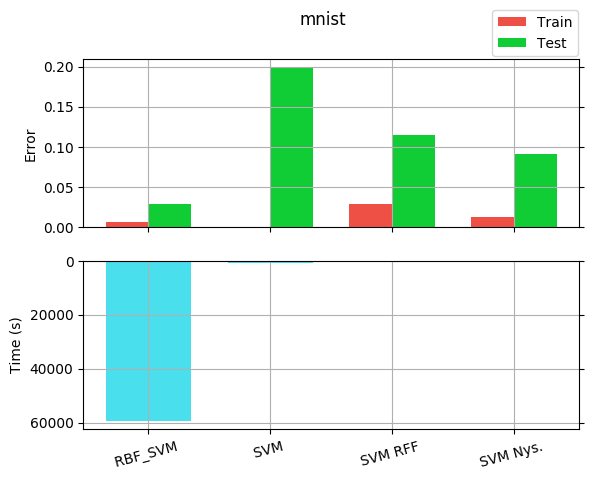
\includegraphics[scale=0.6]{Figures/1_1/mnist}
\decoRule
\caption{Exp. 1.1 with MNIST. SVM is outperformed}
\label{eje:1_1}
\end{figure}


Hypothesis 1 claimed that Linear SVMs could achieve the accuracy of an
RBF-SVM but with much less training time. To check that we ran experiment
1.1, whose results can be seen in \ref{Appendix1-1}.

We can see that the models using Random Fourier Features or \Nys\ (shorted as
RFF and Nys.) reduce the error compared to a single Support Vector Machine
in the cases were using the real RBF kernel increased the
accuracy. In fact, the error incurred is always very close to the one of
RBF-SVM. See Figure \ref{eje:1_1}.

Regarding the training time, we observe that in most of the datasets it was
needed more time to train a single SVM using a random mapping than to train
an SVM with the RBF kernel. The only situations were the random mapping approach
saved us a lot of time is with datasets MNIST and Fashion MNIST.

We suggest that the reason why that happens is that the overhead of using
the random mapping is too big for small datasets compared to using the RBF
kernel, but becomes less relevant with bigger datasets, since the cost of
the random mapping is linear with the number of instances while the cost of the
optimising with the RBF kernel is cubic.

We conclude that the results obtained provide evidence to assert that the
hypothesis 1 is true for large datasets.

\section*{Hypothesis 2}
\label{disc:h2}

\begin{figure}[th]
\centering
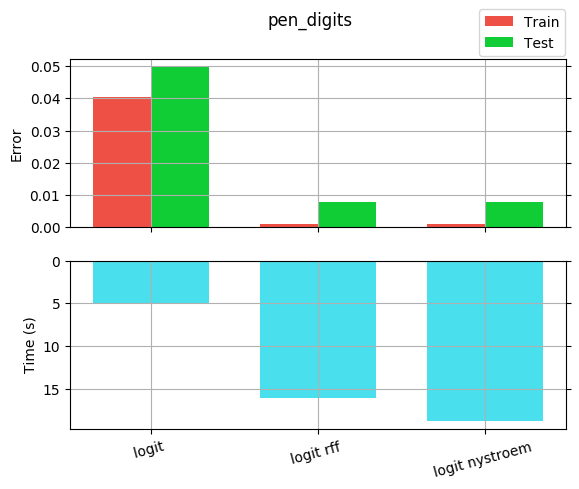
\includegraphics[scale=0.6]{Figures/2_1/pen_digits}
\decoRule
\caption{Exp 2.1 with Pen Digits. Error is decreased by 4\% approx.}
\label{eje:2_1.1}
\end{figure}

\begin{figure}[th]
\centering
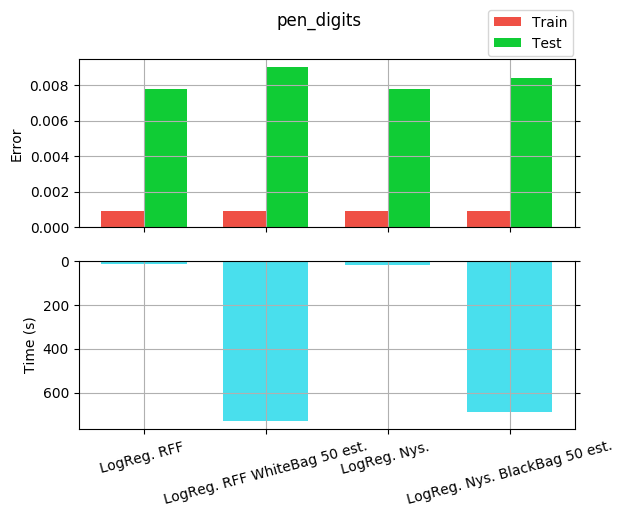
\includegraphics[scale=0.6]{Figures/2_2/aux/pen_digits}
\decoRule
\caption{Logistic Regression with random mapping. A single model vs. an Ensemble. There is not big difference with Pen Digits.}
\label{eje:2_1.2}
\end{figure}

Hypothesis 2 suggested that using a random mapping to train an ensemble of
Logistic Regression models and Support Vector Machines could improve the
accuracy of a single model. To give support to this hypothesis we proposed
the experiments 2.1, 2.2, 2.3 and 2.4. The results of these experiments
can be looked up in
\ref{Appendix2-1},
\ref{Appendix2-2},
\ref{Appendix2-3} and
\ref{Appendix2-4}, respectively.

First, we wanted to see what was the effect of using the random mapping with
a single model, and then with an ensemble.

Experiments \hyperref[Appendix2-1]{2.1} and \hyperref[Appendix2-3]{2.2} were
defined for Logistic Regression.
Except for Fall Detection and Segment, we can see an increase of the accuracy
when using the random mapping on a single estimator. With most of the datasets
the increase is between 2 and 4 \%, and with Vowel it is about 26 \% of
increase. See \ref{eje:2_1.1}.

When used with an ensemble, all of the Box Models show a very similar
improvement to a single estimator.
To see better the differences, they have been put together in a
\hyperref[2_2:aux]{separate chart}. See \ref{eje:2_1.2}
% In \ref{2_2:aux} we can easily
% compare them. Comparació \hyperref[2_2:aux]{aquí}

\hyperref[Appendix2-3]{2.3} and \hyperref[Appendix2-4]{2.4} are the equivalent
experiments for SVM.

With a single model, we can see there is a
meaningful improve in the accuracy
with all datasets except for Fall Detection. The improvements are from 2 \%
(with Digits and Segment) to 35 \% with Vowel.

With an Ensemble of SVMs the increases are more of less the same as with a
single estimator. The differences can be seen in a \hyperref[2_4:aux]{separate
chart}.

Although we can see there are some benefits of using an ensemble of these models,
the training time is a lot higher than with a single one. Given that the
difference between the accuracy of a single model using a random mapping and
an ensemble of them is so tiny, there are not evidences that training an ensemble
of Logistic Regression or SVM with random mapping is worth it. However, in
situations were that tiny difference is very important it could make sense
to use it, specially if one can afford it.
% with the datasets Digits, Pen Digits, and
% Vowel. With the rest of the dataset we can also see some improve, but it is not
% too much.

% Se pueden comparar mejor \hyperref[2_4:aux]{aquí}
\section*{Hypothesis 3}
\label{disc:h3}

\begin{figure}[th]
\centering
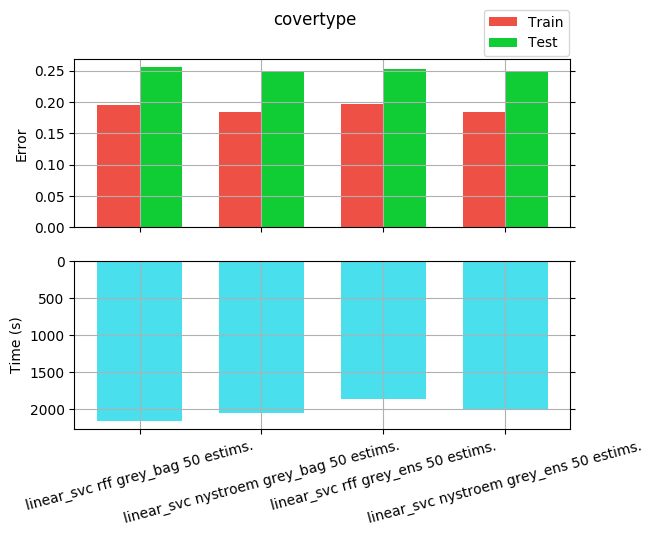
\includegraphics[scale=0.6]{Figures/3_3/covertype}
\decoRule
\caption{Exp. 3.3 with Covertype. White Box Models with Support Vector Machine. There is not much difference between Box Models}
\label{eje:3_1}
\end{figure}

For this hypothesis we expected that the ``Ensemble'' models would get
better results than the ``Bags'' given that Bootstrap with random mapping
could cause too much randomization. To check that we proposed experiments
3.1, 3.2, 3.3 and 3.4. The results can be seen in
\ref{Appendix3-1},
\ref{Appendix3-2},
\ref{Appendix3-3} and
\ref{Appendix3-4}.

In 3.1 we compare the White Box Models with Logistic Regression. It can be seen
that the results are very similar. We can just see a very little improve in using
an Ensemble in Digits, Pen Digits and Vowel (with \Nys).

With the Black Models we can see an improve in more datasets.
Digits, MNIST, Pen Digits, Segment and Vowel present better results with the
Ensemble models.

Regarding the SVMs (in 3.3 and 3.4), the difference is only seen with Vowel,
either in the White and Black Models. See \ref{eje:3_1}.

Based on the results, we can say that whether to perform a bootstrap or not
together with a random mapping doesn't make much difference. However, seen
that Bootstrap does not benefit the models, it may be better to avoid using
it.

\section*{Hypothesis 4}
\label{disc:h4}

\begin{figure}[th]
\centering
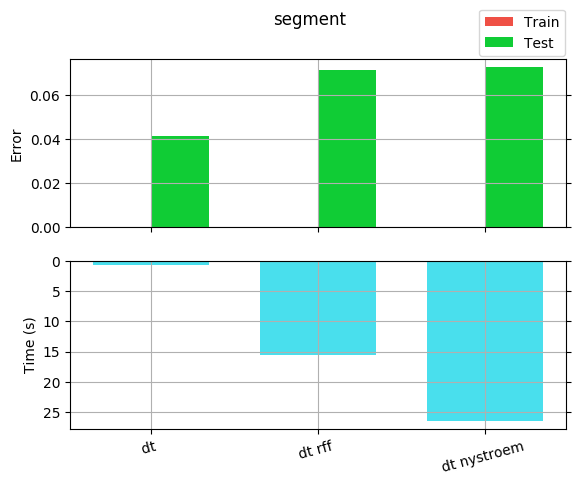
\includegraphics[scale=0.6]{Figures/4_1/segment}
\decoRule
\caption{Exp. 4.1 with Segment. Random Samplers increase the error on Decision Tree.}
\label{eje:4_1}
\end{figure}

\begin{figure}[th]
\centering
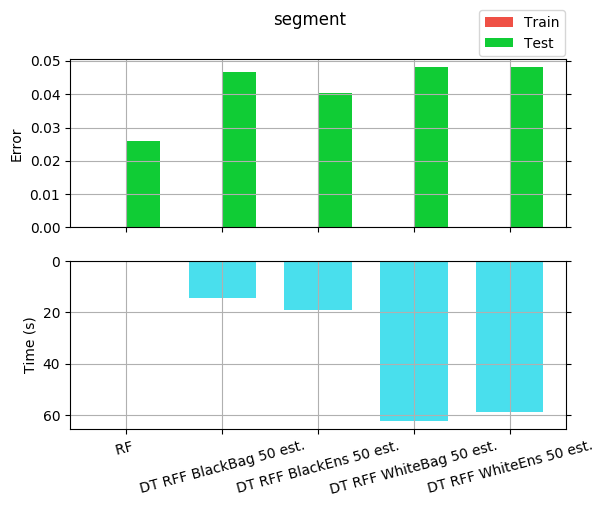
\includegraphics[scale=0.6]{Figures/4_2/rff/segment}
\decoRule
\caption{Exp. 4.2 with Segment. Random Forest outperforms Ensembles of Decision Tree with RFF.}
\label{eje:4_2}
\end{figure}


Hypothesis 4 claimed that Decision Tree could not benefit of using
Random Fourier Features or \Nys. To check that, we proposed experiments
4.1 and 4.2. The first one, which can be seen in \ref{Appendix4-1} was
to compare a single tree, and the second one, in \ref{Appendix4-2}, an
ensemble. For 4.2 a Random Forest was used instead of a Decision Tree since
they benefit with Bagging.

With a single model, we can see no improvement of using a random mapping for
any of the datasets. Besides, the training time is increased. See \ref{eje:4_1}.

With ensembles, however, there is a very little improvement with
Pen Digits and Vowel. But as for the majority of the datasets the error is
increased, we can say that using RFF or \Nys\ with Decision Tree is in
general a bad choice. See \ref{eje:4_2}

We observe there are big differences in the training time of a Random Forest
and the Ensembles of Decision Tree with random mapping. We guess that the
reason for that is that
we used a full-fledged implementation of Random Forest, which may already
by highly optmised, whilst for the Decision Tree we stacked together
many different methods and may have a naive implementation.

% Random Forest is a well known algorithm and it has
% been highly optimised, whilst the Decision Tree have a more straightforward
% procedure which is less efficient.

\end{pre-delivery}

% \begin{note}
%   \section{Enfrentar resultados 2 a 2}
% \end{note}
% \begin{note}
%   \section*{Exp 1-1}
%   \begin{itemize}
%     \item Nunca jamás conseguimos sacar mejores resultados que una RBF-SVM
%     \item Pero los resultados que conseguimos son bastante parecidos en algunos
%     casos
%     \item En el experimento que hamos hecho, los tiempos de los métodos lineales
%     son mucho mayores que los de la RBF-SVM
%     \item Pero hay que atribuirlo al pequeño tamaño del dataset que hemos usado.
%     En un dataset más grande sí se notaría
%     \item Efectivamente, he realizado el experimento en fashion-mnist, y no hay
%     comparación
%   \end{itemize}
%
%   \section*{Exp 2-1}
%   \begin{itemize}
%     \item En general sí conseguimos mejorar sustancialmente un logit
%     \item Pero los tiempos son un poco mayores
%     \item Con datasets mayores, es de esperar que los tiempos no se disparen
%     demasiado
%   \end{itemize}
%
% \section*{Exp 2-2}
% \begin{itemize}
%   \item En los mismos datasets en los que un solo logit no había conseguido hacer
%   nada, aquí tampoco han hecho nada
%   \item Entre logit normal y logit con ensemble, la precisión es más o menos la
%   misma, pero el tiempo es mucho mayor
%   \item En el caso logit, realmente puede deberse a que no hemos hecho nada
%   para sobreajustar más.
% \end{itemize}
%
% \section*{2-3}
% \begin{itemize}
%   \item Exactamente igual que el anterior
% \end{itemize}
%
% \section*{2-4}
% \begin{itemize}
%   \item Exactamente igual que el anterior
% \end{itemize}
%
% \section*{2-5}
% \begin{itemize}
%   \item Conseguimos mejorar sustancialmente la precisión de la mayoría de
%   datasets
%   \item Los tiempos son mayores, pero todavía son aceptables
%   \item Suponemos que en datasets más grandes los tiempo serían más parecidos
% \end{itemize}
%
% \section*{2-6}
% \begin{itemize}
%   \item El dataset que se resistía se sigue resistiendo cuando hacemos un
%   ensemble
%   \item Ahora los tiempo sí que són muchísimo más grandes, quizá no sale a cuenta
%   hacer ensemble
%   \item Para ver si sale a cuenta hacer ensemble, habrá que verlo más adelante
% \end{itemize}
%
% \section*{2-7}
% \begin{itemize}
%   \item Exactamente igual que el anterior
% \end{itemize}
%
% \section*{2-8}
% \begin{itemize}
%   \item Exactamente igual que el anterior
% \end{itemize}
%
% \section*{3-1}
% \begin{itemize}
%   \item No podemos decir que haya una ensemble que claramente sea mejor que los
%   demás
%   \item Da la impresión que en algunos casos el grey es mejor que los otros,
%   pero no es nada concluyente
% \end{itemize}
%
% \section*{3-2}
% \begin{itemize}
%   \item Da la impresión que los black ensembles son un poco mejor que los grey,
%   pero no es nada concluyente
% \end{itemize}
%
% \section*{3-3}
% \begin{itemize}
%   \item Los resultados no son nada concluyentes
% \end{itemize}
%
% \section*{3-4}
% \begin{itemize}
%   \item Exactamente igual que el anterior
% \end{itemize}
%
% \section*{4-1}
% \begin{itemize}
%   \item Usar rff con un solo árbol no es nada beneficioso
%   \item Tanto los errores como los tiempos son más altos
% \end{itemize}
%
% \section*{4-2}
% \begin{itemize}
%   \item En algunos casos ha mejorado sustancialmente, y en otros no
%   \item Pero estamos comparando un solo árbol con 50: claramente los 50
%   tendrían que ser siempre mejores, y ese no es el caso
%   \item Los tiempos no tienen ninguna comparación
%   \item En algunos casos, incluso empeora el usar un ensemble
% \end{itemize}
%
% \section*{4-3}
% \begin{itemize}
%   \item Exactamente igual que el anterior
% \end{itemize}
%
% \section*{4-4}
% \begin{itemize}
%   \item Exactamente igual que el anterior
% \end{itemize}
%
% \section*{4-5}
% \begin{itemize}
%   \item Exactamente igual que el anterior
% \end{itemize}
%
% \end{note}
% \begin{note}
%   \section{Contrastar hipótesis con resultados}
% \end{note}
